\begin{problem}{Tree Product}{\textsl{standard input}}{\textsl{standard output}}{2 seconds}{256 mebibytes}

Given $n$ rooted trees $T_1,T_2,\ldots,T_n$, find two permutations $p_1,p_2,\dots,p_n$ and $q_1,q_2,\ldots,q_n$ such that the diameter of $T_{p_1} \times T_{p_2} \times \ldots \times T_{p_n}$ is maximum and the diameter of $T_{q_1} \times T_{q_2} \times \ldots \times T_{q_n}$ is minimum.

For two rooted trees $A$ and $B$, their \textit{tree product} $T = A \times B$ is defined as follows: copy tree $A$, and then for each vertex $x$ in it, make a copy of $B$ and merge its root with vertex $x$. See the table below for an example:
\begin{center}
\begin{tabular}{cccc}
$A$ & $B$ & $A \times B$ & $B \times A$ \\
\hline \\
\includegraphics[scale=0.5]{tree1.eps} & \includegraphics[scale=0.5]{tree2.eps} & \includegraphics[scale=0.5]{tree4.eps} & \includegraphics[scale=0.5]{tree5.eps}
\end{tabular}
\end{center}

It can be shown that tree product is associative: $(A \times B) \times C = A \times (B \times C)$. So the parentheses in a product of three or more trees can be omitted.

Recall that:

\begin{itemize}
\item A tree is a connected graph without cycles. A rooted tree has a special vertex called the root. The parent of a vertex $v$ is the last vertex different from $v$ on the path from the root to $v$.
\item The diameter of a rooted tree is the length of the longest simple path in the tree, where the length of a path is the number of edges in the path.
\end{itemize}

\InputFile
There are multiple test cases. The first line of input contains an integer $T$, indicating the number of test cases. For each test case:

The first line contains an integer $n$ $(1 \le n \le 10^6)$, indicating the number of rooted trees.

Each of the next $n$ lines starts from an integer $m_i$ ($1 \le m_i \le 10^5$), indicating the number of vertices in the $i$-th rooted tree. It is followed by $m_i$ integers $p_{i,1},p_{i,2},\ldots,p_{i,m_i}$ ($0 \le p_{i,j} \le m_i$) on the same line, where the $j$-th of them denotes the parent of the $j$-th vertex. The root of the tree has $0$ as parent.

It is guaranteed that the sum of $m_i$ over all test cases does not exceed $10^6$.


\OutputFile
For each test case, output two integers: the maximum and the minimum diameter, in that order.




\Example

\begin{example}
\exmpfile{example.01}{example.01.a}%
\end{example}

\Note
For the first sample test case, $T_1 \times T_2 \times T_3$ will provide the maximum diameter, while $T_3 \times T_2 \times T_1$ will provide the minimum diameter.

\end{problem}
